\documentclass[11pt]{article}

    \usepackage[breakable]{tcolorbox}
    \usepackage{parskip} % Stop auto-indenting (to mimic markdown behaviour)
    
    \usepackage{iftex}
    \ifPDFTeX
    	\usepackage[T1]{fontenc}
    	\usepackage{mathpazo}
    \else
    	\usepackage{fontspec}
    \fi

    % Basic figure setup, for now with no caption control since it's done
    % automatically by Pandoc (which extracts ![](path) syntax from Markdown).
    \usepackage{graphicx}
    % Maintain compatibility with old templates. Remove in nbconvert 6.0
    \let\Oldincludegraphics\includegraphics
    % Ensure that by default, figures have no caption (until we provide a
    % proper Figure object with a Caption API and a way to capture that
    % in the conversion process - todo).
    \usepackage{caption}
    \DeclareCaptionFormat{nocaption}{}
    \captionsetup{format=nocaption,aboveskip=0pt,belowskip=0pt}

    \usepackage[Export]{adjustbox} % Used to constrain images to a maximum size
    \adjustboxset{max size={0.9\linewidth}{0.9\paperheight}}
    \usepackage{float}
    \floatplacement{figure}{H} % forces figures to be placed at the correct location
    \usepackage{xcolor} % Allow colors to be defined
    \usepackage{enumerate} % Needed for markdown enumerations to work
    \usepackage{geometry} % Used to adjust the document margins
    \usepackage{amsmath} % Equations
    \usepackage{amssymb} % Equations
    \usepackage{textcomp} % defines textquotesingle
    % Hack from http://tex.stackexchange.com/a/47451/13684:
    \AtBeginDocument{%
        \def\PYZsq{\textquotesingle}% Upright quotes in Pygmentized code
    }
    \usepackage{upquote} % Upright quotes for verbatim code
    \usepackage{eurosym} % defines \euro
    \usepackage[mathletters]{ucs} % Extended unicode (utf-8) support
    \usepackage{fancyvrb} % verbatim replacement that allows latex
    \usepackage{grffile} % extends the file name processing of package graphics 
                         % to support a larger range
    \makeatletter % fix for grffile with XeLaTeX
    \def\Gread@@xetex#1{%
      \IfFileExists{"\Gin@base".bb}%
      {\Gread@eps{\Gin@base.bb}}%
      {\Gread@@xetex@aux#1}%
    }
    \makeatother

    % The hyperref package gives us a pdf with properly built
    % internal navigation ('pdf bookmarks' for the table of contents,
    % internal cross-reference links, web links for URLs, etc.)
    \usepackage{hyperref}
    % The default LaTeX title has an obnoxious amount of whitespace. By default,
    % titling removes some of it. It also provides customization options.
    \usepackage{titling}
    \usepackage{longtable} % longtable support required by pandoc >1.10
    \usepackage{booktabs}  % table support for pandoc > 1.12.2
    \usepackage[inline]{enumitem} % IRkernel/repr support (it uses the enumerate* environment)
    \usepackage[normalem]{ulem} % ulem is needed to support strikethroughs (\sout)
                                % normalem makes italics be italics, not underlines
    \usepackage{mathrsfs}
    

    
    % Colors for the hyperref package
    \definecolor{urlcolor}{rgb}{0,.145,.698}
    \definecolor{linkcolor}{rgb}{.71,0.21,0.01}
    \definecolor{citecolor}{rgb}{.12,.54,.11}

    % ANSI colors
    \definecolor{ansi-black}{HTML}{3E424D}
    \definecolor{ansi-black-intense}{HTML}{282C36}
    \definecolor{ansi-red}{HTML}{E75C58}
    \definecolor{ansi-red-intense}{HTML}{B22B31}
    \definecolor{ansi-green}{HTML}{00A250}
    \definecolor{ansi-green-intense}{HTML}{007427}
    \definecolor{ansi-yellow}{HTML}{DDB62B}
    \definecolor{ansi-yellow-intense}{HTML}{B27D12}
    \definecolor{ansi-blue}{HTML}{208FFB}
    \definecolor{ansi-blue-intense}{HTML}{0065CA}
    \definecolor{ansi-magenta}{HTML}{D160C4}
    \definecolor{ansi-magenta-intense}{HTML}{A03196}
    \definecolor{ansi-cyan}{HTML}{60C6C8}
    \definecolor{ansi-cyan-intense}{HTML}{258F8F}
    \definecolor{ansi-white}{HTML}{C5C1B4}
    \definecolor{ansi-white-intense}{HTML}{A1A6B2}
    \definecolor{ansi-default-inverse-fg}{HTML}{FFFFFF}
    \definecolor{ansi-default-inverse-bg}{HTML}{000000}

    % commands and environments needed by pandoc snippets
    % extracted from the output of `pandoc -s`
    \providecommand{\tightlist}{%
      \setlength{\itemsep}{0pt}\setlength{\parskip}{0pt}}
    \DefineVerbatimEnvironment{Highlighting}{Verbatim}{commandchars=\\\{\}}
    % Add ',fontsize=\small' for more characters per line
    \newenvironment{Shaded}{}{}
    \newcommand{\KeywordTok}[1]{\textcolor[rgb]{0.00,0.44,0.13}{\textbf{{#1}}}}
    \newcommand{\DataTypeTok}[1]{\textcolor[rgb]{0.56,0.13,0.00}{{#1}}}
    \newcommand{\DecValTok}[1]{\textcolor[rgb]{0.25,0.63,0.44}{{#1}}}
    \newcommand{\BaseNTok}[1]{\textcolor[rgb]{0.25,0.63,0.44}{{#1}}}
    \newcommand{\FloatTok}[1]{\textcolor[rgb]{0.25,0.63,0.44}{{#1}}}
    \newcommand{\CharTok}[1]{\textcolor[rgb]{0.25,0.44,0.63}{{#1}}}
    \newcommand{\StringTok}[1]{\textcolor[rgb]{0.25,0.44,0.63}{{#1}}}
    \newcommand{\CommentTok}[1]{\textcolor[rgb]{0.38,0.63,0.69}{\textit{{#1}}}}
    \newcommand{\OtherTok}[1]{\textcolor[rgb]{0.00,0.44,0.13}{{#1}}}
    \newcommand{\AlertTok}[1]{\textcolor[rgb]{1.00,0.00,0.00}{\textbf{{#1}}}}
    \newcommand{\FunctionTok}[1]{\textcolor[rgb]{0.02,0.16,0.49}{{#1}}}
    \newcommand{\RegionMarkerTok}[1]{{#1}}
    \newcommand{\ErrorTok}[1]{\textcolor[rgb]{1.00,0.00,0.00}{\textbf{{#1}}}}
    \newcommand{\NormalTok}[1]{{#1}}
    
    % Additional commands for more recent versions of Pandoc
    \newcommand{\ConstantTok}[1]{\textcolor[rgb]{0.53,0.00,0.00}{{#1}}}
    \newcommand{\SpecialCharTok}[1]{\textcolor[rgb]{0.25,0.44,0.63}{{#1}}}
    \newcommand{\VerbatimStringTok}[1]{\textcolor[rgb]{0.25,0.44,0.63}{{#1}}}
    \newcommand{\SpecialStringTok}[1]{\textcolor[rgb]{0.73,0.40,0.53}{{#1}}}
    \newcommand{\ImportTok}[1]{{#1}}
    \newcommand{\DocumentationTok}[1]{\textcolor[rgb]{0.73,0.13,0.13}{\textit{{#1}}}}
    \newcommand{\AnnotationTok}[1]{\textcolor[rgb]{0.38,0.63,0.69}{\textbf{\textit{{#1}}}}}
    \newcommand{\CommentVarTok}[1]{\textcolor[rgb]{0.38,0.63,0.69}{\textbf{\textit{{#1}}}}}
    \newcommand{\VariableTok}[1]{\textcolor[rgb]{0.10,0.09,0.49}{{#1}}}
    \newcommand{\ControlFlowTok}[1]{\textcolor[rgb]{0.00,0.44,0.13}{\textbf{{#1}}}}
    \newcommand{\OperatorTok}[1]{\textcolor[rgb]{0.40,0.40,0.40}{{#1}}}
    \newcommand{\BuiltInTok}[1]{{#1}}
    \newcommand{\ExtensionTok}[1]{{#1}}
    \newcommand{\PreprocessorTok}[1]{\textcolor[rgb]{0.74,0.48,0.00}{{#1}}}
    \newcommand{\AttributeTok}[1]{\textcolor[rgb]{0.49,0.56,0.16}{{#1}}}
    \newcommand{\InformationTok}[1]{\textcolor[rgb]{0.38,0.63,0.69}{\textbf{\textit{{#1}}}}}
    \newcommand{\WarningTok}[1]{\textcolor[rgb]{0.38,0.63,0.69}{\textbf{\textit{{#1}}}}}
    
    
    % Define a nice break command that doesn't care if a line doesn't already
    % exist.
    \def\br{\hspace*{\fill} \\* }
    % Math Jax compatibility definitions
    \def\gt{>}
    \def\lt{<}
    \let\Oldtex\TeX
    \let\Oldlatex\LaTeX
    \renewcommand{\TeX}{\textrm{\Oldtex}}
    \renewcommand{\LaTeX}{\textrm{\Oldlatex}}
    % Document parameters
    % Document title
    \title{Knowledge Graphs Demystified Part 2: Practical Session}
    \date{15 April 2021}
    
    
    
    
    
% Pygments definitions
\makeatletter
\def\PY@reset{\let\PY@it=\relax \let\PY@bf=\relax%
    \let\PY@ul=\relax \let\PY@tc=\relax%
    \let\PY@bc=\relax \let\PY@ff=\relax}
\def\PY@tok#1{\csname PY@tok@#1\endcsname}
\def\PY@toks#1+{\ifx\relax#1\empty\else%
    \PY@tok{#1}\expandafter\PY@toks\fi}
\def\PY@do#1{\PY@bc{\PY@tc{\PY@ul{%
    \PY@it{\PY@bf{\PY@ff{#1}}}}}}}
\def\PY#1#2{\PY@reset\PY@toks#1+\relax+\PY@do{#2}}

\expandafter\def\csname PY@tok@w\endcsname{\def\PY@tc##1{\textcolor[rgb]{0.73,0.73,0.73}{##1}}}
\expandafter\def\csname PY@tok@c\endcsname{\let\PY@it=\textit\def\PY@tc##1{\textcolor[rgb]{0.25,0.50,0.50}{##1}}}
\expandafter\def\csname PY@tok@cp\endcsname{\def\PY@tc##1{\textcolor[rgb]{0.74,0.48,0.00}{##1}}}
\expandafter\def\csname PY@tok@k\endcsname{\let\PY@bf=\textbf\def\PY@tc##1{\textcolor[rgb]{0.00,0.50,0.00}{##1}}}
\expandafter\def\csname PY@tok@kp\endcsname{\def\PY@tc##1{\textcolor[rgb]{0.00,0.50,0.00}{##1}}}
\expandafter\def\csname PY@tok@kt\endcsname{\def\PY@tc##1{\textcolor[rgb]{0.69,0.00,0.25}{##1}}}
\expandafter\def\csname PY@tok@o\endcsname{\def\PY@tc##1{\textcolor[rgb]{0.40,0.40,0.40}{##1}}}
\expandafter\def\csname PY@tok@ow\endcsname{\let\PY@bf=\textbf\def\PY@tc##1{\textcolor[rgb]{0.67,0.13,1.00}{##1}}}
\expandafter\def\csname PY@tok@nb\endcsname{\def\PY@tc##1{\textcolor[rgb]{0.00,0.50,0.00}{##1}}}
\expandafter\def\csname PY@tok@nf\endcsname{\def\PY@tc##1{\textcolor[rgb]{0.00,0.00,1.00}{##1}}}
\expandafter\def\csname PY@tok@nc\endcsname{\let\PY@bf=\textbf\def\PY@tc##1{\textcolor[rgb]{0.00,0.00,1.00}{##1}}}
\expandafter\def\csname PY@tok@nn\endcsname{\let\PY@bf=\textbf\def\PY@tc##1{\textcolor[rgb]{0.00,0.00,1.00}{##1}}}
\expandafter\def\csname PY@tok@ne\endcsname{\let\PY@bf=\textbf\def\PY@tc##1{\textcolor[rgb]{0.82,0.25,0.23}{##1}}}
\expandafter\def\csname PY@tok@nv\endcsname{\def\PY@tc##1{\textcolor[rgb]{0.10,0.09,0.49}{##1}}}
\expandafter\def\csname PY@tok@no\endcsname{\def\PY@tc##1{\textcolor[rgb]{0.53,0.00,0.00}{##1}}}
\expandafter\def\csname PY@tok@nl\endcsname{\def\PY@tc##1{\textcolor[rgb]{0.63,0.63,0.00}{##1}}}
\expandafter\def\csname PY@tok@ni\endcsname{\let\PY@bf=\textbf\def\PY@tc##1{\textcolor[rgb]{0.60,0.60,0.60}{##1}}}
\expandafter\def\csname PY@tok@na\endcsname{\def\PY@tc##1{\textcolor[rgb]{0.49,0.56,0.16}{##1}}}
\expandafter\def\csname PY@tok@nt\endcsname{\let\PY@bf=\textbf\def\PY@tc##1{\textcolor[rgb]{0.00,0.50,0.00}{##1}}}
\expandafter\def\csname PY@tok@nd\endcsname{\def\PY@tc##1{\textcolor[rgb]{0.67,0.13,1.00}{##1}}}
\expandafter\def\csname PY@tok@s\endcsname{\def\PY@tc##1{\textcolor[rgb]{0.73,0.13,0.13}{##1}}}
\expandafter\def\csname PY@tok@sd\endcsname{\let\PY@it=\textit\def\PY@tc##1{\textcolor[rgb]{0.73,0.13,0.13}{##1}}}
\expandafter\def\csname PY@tok@si\endcsname{\let\PY@bf=\textbf\def\PY@tc##1{\textcolor[rgb]{0.73,0.40,0.53}{##1}}}
\expandafter\def\csname PY@tok@se\endcsname{\let\PY@bf=\textbf\def\PY@tc##1{\textcolor[rgb]{0.73,0.40,0.13}{##1}}}
\expandafter\def\csname PY@tok@sr\endcsname{\def\PY@tc##1{\textcolor[rgb]{0.73,0.40,0.53}{##1}}}
\expandafter\def\csname PY@tok@ss\endcsname{\def\PY@tc##1{\textcolor[rgb]{0.10,0.09,0.49}{##1}}}
\expandafter\def\csname PY@tok@sx\endcsname{\def\PY@tc##1{\textcolor[rgb]{0.00,0.50,0.00}{##1}}}
\expandafter\def\csname PY@tok@m\endcsname{\def\PY@tc##1{\textcolor[rgb]{0.40,0.40,0.40}{##1}}}
\expandafter\def\csname PY@tok@gh\endcsname{\let\PY@bf=\textbf\def\PY@tc##1{\textcolor[rgb]{0.00,0.00,0.50}{##1}}}
\expandafter\def\csname PY@tok@gu\endcsname{\let\PY@bf=\textbf\def\PY@tc##1{\textcolor[rgb]{0.50,0.00,0.50}{##1}}}
\expandafter\def\csname PY@tok@gd\endcsname{\def\PY@tc##1{\textcolor[rgb]{0.63,0.00,0.00}{##1}}}
\expandafter\def\csname PY@tok@gi\endcsname{\def\PY@tc##1{\textcolor[rgb]{0.00,0.63,0.00}{##1}}}
\expandafter\def\csname PY@tok@gr\endcsname{\def\PY@tc##1{\textcolor[rgb]{1.00,0.00,0.00}{##1}}}
\expandafter\def\csname PY@tok@ge\endcsname{\let\PY@it=\textit}
\expandafter\def\csname PY@tok@gs\endcsname{\let\PY@bf=\textbf}
\expandafter\def\csname PY@tok@gp\endcsname{\let\PY@bf=\textbf\def\PY@tc##1{\textcolor[rgb]{0.00,0.00,0.50}{##1}}}
\expandafter\def\csname PY@tok@go\endcsname{\def\PY@tc##1{\textcolor[rgb]{0.53,0.53,0.53}{##1}}}
\expandafter\def\csname PY@tok@gt\endcsname{\def\PY@tc##1{\textcolor[rgb]{0.00,0.27,0.87}{##1}}}
\expandafter\def\csname PY@tok@err\endcsname{\def\PY@bc##1{\setlength{\fboxsep}{0pt}\fcolorbox[rgb]{1.00,0.00,0.00}{1,1,1}{\strut ##1}}}
\expandafter\def\csname PY@tok@kc\endcsname{\let\PY@bf=\textbf\def\PY@tc##1{\textcolor[rgb]{0.00,0.50,0.00}{##1}}}
\expandafter\def\csname PY@tok@kd\endcsname{\let\PY@bf=\textbf\def\PY@tc##1{\textcolor[rgb]{0.00,0.50,0.00}{##1}}}
\expandafter\def\csname PY@tok@kn\endcsname{\let\PY@bf=\textbf\def\PY@tc##1{\textcolor[rgb]{0.00,0.50,0.00}{##1}}}
\expandafter\def\csname PY@tok@kr\endcsname{\let\PY@bf=\textbf\def\PY@tc##1{\textcolor[rgb]{0.00,0.50,0.00}{##1}}}
\expandafter\def\csname PY@tok@bp\endcsname{\def\PY@tc##1{\textcolor[rgb]{0.00,0.50,0.00}{##1}}}
\expandafter\def\csname PY@tok@fm\endcsname{\def\PY@tc##1{\textcolor[rgb]{0.00,0.00,1.00}{##1}}}
\expandafter\def\csname PY@tok@vc\endcsname{\def\PY@tc##1{\textcolor[rgb]{0.10,0.09,0.49}{##1}}}
\expandafter\def\csname PY@tok@vg\endcsname{\def\PY@tc##1{\textcolor[rgb]{0.10,0.09,0.49}{##1}}}
\expandafter\def\csname PY@tok@vi\endcsname{\def\PY@tc##1{\textcolor[rgb]{0.10,0.09,0.49}{##1}}}
\expandafter\def\csname PY@tok@vm\endcsname{\def\PY@tc##1{\textcolor[rgb]{0.10,0.09,0.49}{##1}}}
\expandafter\def\csname PY@tok@sa\endcsname{\def\PY@tc##1{\textcolor[rgb]{0.73,0.13,0.13}{##1}}}
\expandafter\def\csname PY@tok@sb\endcsname{\def\PY@tc##1{\textcolor[rgb]{0.73,0.13,0.13}{##1}}}
\expandafter\def\csname PY@tok@sc\endcsname{\def\PY@tc##1{\textcolor[rgb]{0.73,0.13,0.13}{##1}}}
\expandafter\def\csname PY@tok@dl\endcsname{\def\PY@tc##1{\textcolor[rgb]{0.73,0.13,0.13}{##1}}}
\expandafter\def\csname PY@tok@s2\endcsname{\def\PY@tc##1{\textcolor[rgb]{0.73,0.13,0.13}{##1}}}
\expandafter\def\csname PY@tok@sh\endcsname{\def\PY@tc##1{\textcolor[rgb]{0.73,0.13,0.13}{##1}}}
\expandafter\def\csname PY@tok@s1\endcsname{\def\PY@tc##1{\textcolor[rgb]{0.73,0.13,0.13}{##1}}}
\expandafter\def\csname PY@tok@mb\endcsname{\def\PY@tc##1{\textcolor[rgb]{0.40,0.40,0.40}{##1}}}
\expandafter\def\csname PY@tok@mf\endcsname{\def\PY@tc##1{\textcolor[rgb]{0.40,0.40,0.40}{##1}}}
\expandafter\def\csname PY@tok@mh\endcsname{\def\PY@tc##1{\textcolor[rgb]{0.40,0.40,0.40}{##1}}}
\expandafter\def\csname PY@tok@mi\endcsname{\def\PY@tc##1{\textcolor[rgb]{0.40,0.40,0.40}{##1}}}
\expandafter\def\csname PY@tok@il\endcsname{\def\PY@tc##1{\textcolor[rgb]{0.40,0.40,0.40}{##1}}}
\expandafter\def\csname PY@tok@mo\endcsname{\def\PY@tc##1{\textcolor[rgb]{0.40,0.40,0.40}{##1}}}
\expandafter\def\csname PY@tok@ch\endcsname{\let\PY@it=\textit\def\PY@tc##1{\textcolor[rgb]{0.25,0.50,0.50}{##1}}}
\expandafter\def\csname PY@tok@cm\endcsname{\let\PY@it=\textit\def\PY@tc##1{\textcolor[rgb]{0.25,0.50,0.50}{##1}}}
\expandafter\def\csname PY@tok@cpf\endcsname{\let\PY@it=\textit\def\PY@tc##1{\textcolor[rgb]{0.25,0.50,0.50}{##1}}}
\expandafter\def\csname PY@tok@c1\endcsname{\let\PY@it=\textit\def\PY@tc##1{\textcolor[rgb]{0.25,0.50,0.50}{##1}}}
\expandafter\def\csname PY@tok@cs\endcsname{\let\PY@it=\textit\def\PY@tc##1{\textcolor[rgb]{0.25,0.50,0.50}{##1}}}

\def\PYZbs{\char`\\}
\def\PYZus{\char`\_}
\def\PYZob{\char`\{}
\def\PYZcb{\char`\}}
\def\PYZca{\char`\^}
\def\PYZam{\char`\&}
\def\PYZlt{\char`\<}
\def\PYZgt{\char`\>}
\def\PYZsh{\char`\#}
\def\PYZpc{\char`\%}
\def\PYZdl{\char`\$}
\def\PYZhy{\char`\-}
\def\PYZsq{\char`\'}
\def\PYZdq{\char`\"}
\def\PYZti{\char`\~}
% for compatibility with earlier versions
\def\PYZat{@}
\def\PYZlb{[}
\def\PYZrb{]}
\makeatother


    % For linebreaks inside Verbatim environment from package fancyvrb. 
    \makeatletter
        \newbox\Wrappedcontinuationbox 
        \newbox\Wrappedvisiblespacebox 
        \newcommand*\Wrappedvisiblespace {\textcolor{red}{\textvisiblespace}} 
        \newcommand*\Wrappedcontinuationsymbol {\textcolor{red}{\llap{\tiny$\m@th\hookrightarrow$}}} 
        \newcommand*\Wrappedcontinuationindent {3ex } 
        \newcommand*\Wrappedafterbreak {\kern\Wrappedcontinuationindent\copy\Wrappedcontinuationbox} 
        % Take advantage of the already applied Pygments mark-up to insert 
        % potential linebreaks for TeX processing. 
        %        {, <, #, %, $, ' and ": go to next line. 
        %        _, }, ^, &, >, - and ~: stay at end of broken line. 
        % Use of \textquotesingle for straight quote. 
        \newcommand*\Wrappedbreaksatspecials {% 
            \def\PYGZus{\discretionary{\char`\_}{\Wrappedafterbreak}{\char`\_}}% 
            \def\PYGZob{\discretionary{}{\Wrappedafterbreak\char`\{}{\char`\{}}% 
            \def\PYGZcb{\discretionary{\char`\}}{\Wrappedafterbreak}{\char`\}}}% 
            \def\PYGZca{\discretionary{\char`\^}{\Wrappedafterbreak}{\char`\^}}% 
            \def\PYGZam{\discretionary{\char`\&}{\Wrappedafterbreak}{\char`\&}}% 
            \def\PYGZlt{\discretionary{}{\Wrappedafterbreak\char`\<}{\char`\<}}% 
            \def\PYGZgt{\discretionary{\char`\>}{\Wrappedafterbreak}{\char`\>}}% 
            \def\PYGZsh{\discretionary{}{\Wrappedafterbreak\char`\#}{\char`\#}}% 
            \def\PYGZpc{\discretionary{}{\Wrappedafterbreak\char`\%}{\char`\%}}% 
            \def\PYGZdl{\discretionary{}{\Wrappedafterbreak\char`\$}{\char`\$}}% 
            \def\PYGZhy{\discretionary{\char`\-}{\Wrappedafterbreak}{\char`\-}}% 
            \def\PYGZsq{\discretionary{}{\Wrappedafterbreak\textquotesingle}{\textquotesingle}}% 
            \def\PYGZdq{\discretionary{}{\Wrappedafterbreak\char`\"}{\char`\"}}% 
            \def\PYGZti{\discretionary{\char`\~}{\Wrappedafterbreak}{\char`\~}}% 
        } 
        % Some characters . , ; ? ! / are not pygmentized. 
        % This macro makes them "active" and they will insert potential linebreaks 
        \newcommand*\Wrappedbreaksatpunct {% 
            \lccode`\~`\.\lowercase{\def~}{\discretionary{\hbox{\char`\.}}{\Wrappedafterbreak}{\hbox{\char`\.}}}% 
            \lccode`\~`\,\lowercase{\def~}{\discretionary{\hbox{\char`\,}}{\Wrappedafterbreak}{\hbox{\char`\,}}}% 
            \lccode`\~`\;\lowercase{\def~}{\discretionary{\hbox{\char`\;}}{\Wrappedafterbreak}{\hbox{\char`\;}}}% 
            \lccode`\~`\:\lowercase{\def~}{\discretionary{\hbox{\char`\:}}{\Wrappedafterbreak}{\hbox{\char`\:}}}% 
            \lccode`\~`\?\lowercase{\def~}{\discretionary{\hbox{\char`\?}}{\Wrappedafterbreak}{\hbox{\char`\?}}}% 
            \lccode`\~`\!\lowercase{\def~}{\discretionary{\hbox{\char`\!}}{\Wrappedafterbreak}{\hbox{\char`\!}}}% 
            \lccode`\~`\/\lowercase{\def~}{\discretionary{\hbox{\char`\/}}{\Wrappedafterbreak}{\hbox{\char`\/}}}% 
            \catcode`\.\active
            \catcode`\,\active 
            \catcode`\;\active
            \catcode`\:\active
            \catcode`\?\active
            \catcode`\!\active
            \catcode`\/\active 
            \lccode`\~`\~ 	
        }
    \makeatother

    \let\OriginalVerbatim=\Verbatim
    \makeatletter
    \renewcommand{\Verbatim}[1][1]{%
        %\parskip\z@skip
        \sbox\Wrappedcontinuationbox {\Wrappedcontinuationsymbol}%
        \sbox\Wrappedvisiblespacebox {\FV@SetupFont\Wrappedvisiblespace}%
        \def\FancyVerbFormatLine ##1{\hsize\linewidth
            \vtop{\raggedright\hyphenpenalty\z@\exhyphenpenalty\z@
                \doublehyphendemerits\z@\finalhyphendemerits\z@
                \strut ##1\strut}%
        }%
        % If the linebreak is at a space, the latter will be displayed as visible
        % space at end of first line, and a continuation symbol starts next line.
        % Stretch/shrink are however usually zero for typewriter font.
        \def\FV@Space {%
            \nobreak\hskip\z@ plus\fontdimen3\font minus\fontdimen4\font
            \discretionary{\copy\Wrappedvisiblespacebox}{\Wrappedafterbreak}
            {\kern\fontdimen2\font}%
        }%
        
        % Allow breaks at special characters using \PYG... macros.
        \Wrappedbreaksatspecials
        % Breaks at punctuation characters . , ; ? ! and / need catcode=\active 	
        \OriginalVerbatim[#1,codes*=\Wrappedbreaksatpunct]%
    }
    \makeatother

    % Exact colors from NB
    \definecolor{incolor}{HTML}{303F9F}
    \definecolor{outcolor}{HTML}{D84315}
    \definecolor{cellborder}{HTML}{CFCFCF}
    \definecolor{cellbackground}{HTML}{F7F7F7}
    
    % prompt
    \makeatletter
    \newcommand{\boxspacing}{\kern\kvtcb@left@rule\kern\kvtcb@boxsep}
    \makeatother
    \newcommand{\prompt}[4]{
        \ttfamily\llap{{\color{#2}[#3]:\hspace{3pt}#4}}\vspace{-\baselineskip}
    }
    

    
    % Prevent overflowing lines due to hard-to-break entities
    \sloppy 
    % Setup hyperref package
    \hypersetup{
      breaklinks=true,  % so long urls are correctly broken across lines
      colorlinks=true,
      urlcolor=urlcolor,
      linkcolor=linkcolor,
      citecolor=citecolor,
      }
    % Slightly bigger margins than the latex defaults
    
    \geometry{verbose,tmargin=1in,bmargin=1in,lmargin=1in,rmargin=1in}
    
    

\begin{document}
    
    \maketitle
    
    

    
    In this notebook we are going to construct a simple knowledge graph
using Python, and run some queries on the graph in Neo4j.

If you would like to run this code yourself, you will need to install
the \texttt{py2neo} package in Python 3.

To run part 3 onwards, you will need to install Neo4j, which can be
downloaded at https://neo4j.com/download/.

I will be running through the code during part 2 of the master class so
there is no need to install anything unless you would also like to try
the code out yourself and run some graph queries.

\hypertarget{read-in-the-data}{%
\section{Read in the data}\label{read-in-the-data}}

Before we can build a graph, we must first read in the example datasets:

\begin{itemize}
\tightlist
\item
  \texttt{work\_order\_file}: A csv file containing a set of work
  orders.
\item
  \texttt{downtime\_file}: a csv file containing a set of downtime
  events.
\end{itemize}

Here is an example of what the first few rows of each dataset look like:

\begin{figure}
\centering
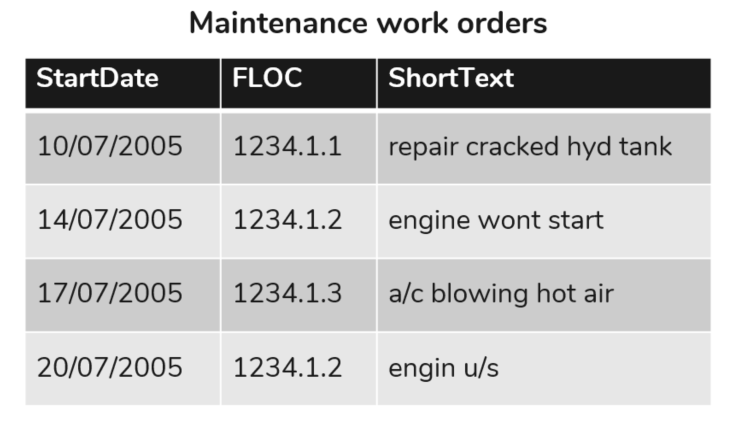
\includegraphics{images/example-data.png}
\caption{alt text}
\end{figure}

We are using the simple \texttt{csv} library to read in the data, though
this can also be done using \texttt{pandas}.

    \begin{tcolorbox}[breakable, size=fbox, boxrule=1pt, pad at break*=1mm,colback=cellbackground, colframe=cellborder]
\prompt{In}{incolor}{73}{\boxspacing}
\begin{Verbatim}[commandchars=\\\{\}]
\PY{k+kn}{from} \PY{n+nn}{csv} \PY{k}{import} \PY{n}{DictReader}

\PY{n}{work\PYZus{}order\PYZus{}file} \PY{o}{=} \PY{l+s+s2}{\PYZdq{}}\PY{l+s+s2}{data/sample\PYZus{}work\PYZus{}orders.csv}\PY{l+s+s2}{\PYZdq{}}
\PY{n}{downtime\PYZus{}file} \PY{o}{=} \PY{l+s+s2}{\PYZdq{}}\PY{l+s+s2}{data/sample\PYZus{}downtime\PYZus{}events.csv}\PY{l+s+s2}{\PYZdq{}}

\PY{c+c1}{\PYZsh{} A simple function to read in a csv file and return a list,}
\PY{c+c1}{\PYZsh{} where each element in the list is a dictionary of \PYZob{}heading : value\PYZcb{}}
\PY{k}{def} \PY{n+nf}{load\PYZus{}csv}\PY{p}{(}\PY{n}{filename}\PY{p}{)}\PY{p}{:}
    \PY{n}{data} \PY{o}{=} \PY{p}{[}\PY{p}{]}
    \PY{k}{with} \PY{n+nb}{open}\PY{p}{(}\PY{n}{filename}\PY{p}{,} \PY{l+s+s1}{\PYZsq{}}\PY{l+s+s1}{r}\PY{l+s+s1}{\PYZsq{}}\PY{p}{)} \PY{k}{as} \PY{n}{f}\PY{p}{:}
        \PY{n}{reader} \PY{o}{=} \PY{n}{DictReader}\PY{p}{(}\PY{n}{f}\PY{p}{)}
        \PY{k}{for} \PY{n}{row} \PY{o+ow}{in} \PY{n}{reader}\PY{p}{:}
            \PY{n}{data}\PY{o}{.}\PY{n}{append}\PY{p}{(}\PY{n}{row}\PY{p}{)}
    \PY{k}{return} \PY{n}{data}

        
\PY{n}{work\PYZus{}order\PYZus{}data} \PY{o}{=} \PY{n}{load\PYZus{}csv}\PY{p}{(}\PY{n}{work\PYZus{}order\PYZus{}file}\PY{p}{)}
\PY{n}{downtime\PYZus{}data} \PY{o}{=} \PY{n}{load\PYZus{}csv}\PY{p}{(}\PY{n}{downtime\PYZus{}file}\PY{p}{)}

\PY{k}{for} \PY{n}{row} \PY{o+ow}{in} \PY{n}{work\PYZus{}order\PYZus{}data}\PY{p}{:}
    \PY{n+nb}{print}\PY{p}{(}\PY{n}{row}\PY{p}{)}

    
\end{Verbatim}
\end{tcolorbox}

    \begin{Verbatim}[commandchars=\\\{\}]
OrderedDict([('StartDate', '10/07/2005'), ('FLOC', '1234.1.1'), ('ShortText',
'repair cracked hyd tank')])
OrderedDict([('StartDate', '14/07/2005'), ('FLOC', '1234.1.2'), ('ShortText',
'engine wont start')])
OrderedDict([('StartDate', '17/07/2005'), ('FLOC', '1234.1.3'), ('ShortText',
'a/c blowing hot air')])
OrderedDict([('StartDate', '20/07/2005'), ('FLOC', '1234.1.2'), ('ShortText',
'engin u/s')])
OrderedDict([('StartDate', '21/07/2005'), ('FLOC', '1234.1.2'), ('ShortText',
'fix engine')])
OrderedDict([('StartDate', '22/07/2005'), ('FLOC', '1234.1.4'), ('ShortText',
'pump service')])
OrderedDict([('StartDate', '23/07/2005'), ('FLOC', '1234.1.4'), ('ShortText',
'pump leak')])
OrderedDict([('StartDate', '24/07/2005'), ('FLOC', '1234.1.4'), ('ShortText',
'fix leak on pump')])
OrderedDict([('StartDate', '25/07/2005'), ('FLOC', '1234.1.2'), ('ShortText',
'engine not running')])
OrderedDict([('StartDate', '26/07/2005'), ('FLOC', '1234.1.2'), ('ShortText',
'engine has problems starting')])
OrderedDict([('StartDate', '27/07/2005'), ('FLOC', '1234.1.4'), ('ShortText',
'pump fault')])
OrderedDict([('StartDate', '28/07/2005'), ('FLOC', '1234.1.4'), ('ShortText',
'pump leaking')])
OrderedDict([('StartDate', '29/07/2005'), ('FLOC', '1234.1.3'), ('ShortText',
'a/c not working')])
OrderedDict([('StartDate', '30/07/2005'), ('FLOC', '1234.1.3'), ('ShortText',
'a/c broken')])
    \end{Verbatim}

    \hypertarget{construct-nodes-from-the-entities-in-the-short-text}{%
\section{Construct nodes from the entities in the short
text}\label{construct-nodes-from-the-entities-in-the-short-text}}

Our first task is to extract the entities in the short text descriptions
and construct nodes from those entities. This is how we are able to
unlock the knowledge captured within the short text and combine it with
the structured fields.

\begin{figure}
\centering
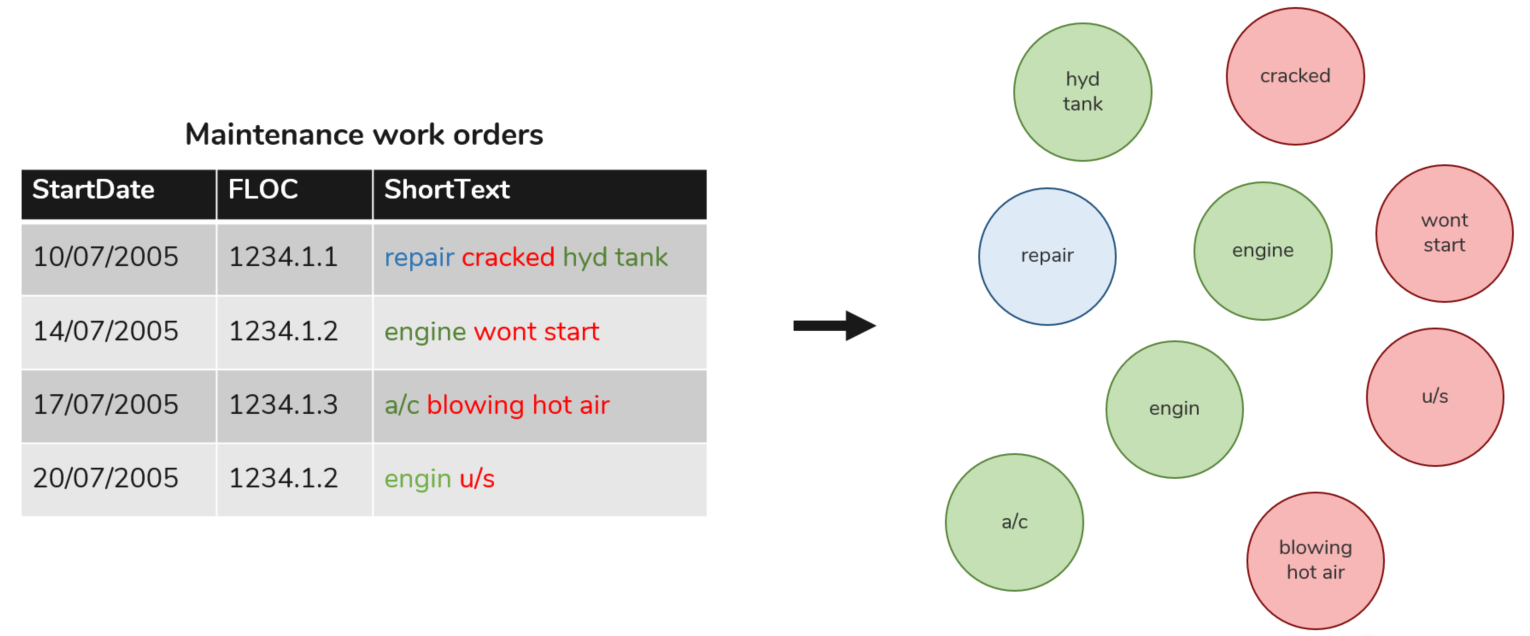
\includegraphics{images/extracting-entities-v2.png}
\caption{alt text}
\end{figure}

    \hypertarget{define-a-lexicon-tagger-class}{%
\subsection{Define a Lexicon Tagger
class}\label{define-a-lexicon-tagger-class}}

Extracting the entities in the short text is typically done using a
trained Named Entity Recognition model, however for simplicity we will
use a Lexicon.

The LexiconTagger class is a simple alternative to a trained named
entity recognition model such as an LSTM or Transformer.

This class serves to automatically extract entities from each sentence
using a predefined lexicon.

    \begin{tcolorbox}[breakable, size=fbox, boxrule=1pt, pad at break*=1mm,colback=cellbackground, colframe=cellborder]
\prompt{In}{incolor}{74}{\boxspacing}
\begin{Verbatim}[commandchars=\\\{\}]
\PY{c+c1}{\PYZsh{} Load the lexicon}

\PY{k+kn}{import} \PY{n+nn}{itertools}

\PY{k}{class} \PY{n+nc}{LexiconTagger}\PY{p}{:}
    \PY{l+s+sd}{\PYZdq{}\PYZdq{}\PYZdq{} A lexicon\PYZhy{}based entity tagger.}
\PY{l+s+sd}{    }
\PY{l+s+sd}{    Args:}
\PY{l+s+sd}{        lexicon\PYZus{}file: The filename of the lexicon.}
\PY{l+s+sd}{    }
\PY{l+s+sd}{    \PYZdq{}\PYZdq{}\PYZdq{}}
    \PY{k}{def} \PY{n+nf}{\PYZus{}\PYZus{}init\PYZus{}\PYZus{}}\PY{p}{(}\PY{n+nb+bp}{self}\PY{p}{,} \PY{n}{lexicon\PYZus{}file}\PY{p}{,} \PY{n}{max\PYZus{}ngram\PYZus{}size} \PY{o}{=} \PY{l+m+mi}{3}\PY{p}{)}\PY{p}{:}
        
        \PY{n}{lexicon\PYZus{}data} \PY{o}{=} \PY{n}{load\PYZus{}csv}\PY{p}{(}\PY{n}{lexicon\PYZus{}file}\PY{p}{)}
        \PY{n+nb+bp}{self}\PY{o}{.}\PY{n}{max\PYZus{}ngram\PYZus{}size} \PY{o}{=} \PY{n}{max\PYZus{}ngram\PYZus{}size}
        
        \PY{c+c1}{\PYZsh{} Convert the loaded csv into a dictionary mapping word(s) to entity class}
        \PY{n+nb+bp}{self}\PY{o}{.}\PY{n}{lexicon} \PY{o}{=} \PY{p}{\PYZob{}}\PY{p}{\PYZcb{}}
        \PY{k}{for} \PY{n}{row} \PY{o+ow}{in} \PY{n}{lexicon\PYZus{}data}\PY{p}{:}
            \PY{n+nb+bp}{self}\PY{o}{.}\PY{n}{lexicon}\PY{p}{[}\PY{n}{row}\PY{p}{[}\PY{l+s+s2}{\PYZdq{}}\PY{l+s+s2}{key}\PY{l+s+s2}{\PYZdq{}}\PY{p}{]}\PY{p}{]} \PY{o}{=} \PY{n}{row}\PY{p}{[}\PY{l+s+s2}{\PYZdq{}}\PY{l+s+s2}{value}\PY{l+s+s2}{\PYZdq{}}\PY{p}{]}      
        
        
    
    \PY{k}{def} \PY{n+nf}{get\PYZus{}ngrams}\PY{p}{(}\PY{n+nb+bp}{self}\PY{p}{,} \PY{n}{sentence}\PY{p}{)}\PY{p}{:}        
        \PY{l+s+sd}{\PYZdq{}\PYZdq{}\PYZdq{}}
\PY{l+s+sd}{            Given a sentence, return a list of all combinations of ngrams up to a certain size.}
\PY{l+s+sd}{            }
\PY{l+s+sd}{            Args:}
\PY{l+s+sd}{                sentence: A list of words, e.g. [\PYZdq{}fix\PYZdq{}, \PYZdq{}broken\PYZdq{}, \PYZdq{}pump\PYZdq{}].}
\PY{l+s+sd}{                }
\PY{l+s+sd}{            Returns:}
\PY{l+s+sd}{                ngrams: A list of ngrams containing up to max\PYZus{}ngram\PYZus{}size words.}
\PY{l+s+sd}{                        For example, given the input [\PYZdq{}fix\PYZdq{}, \PYZdq{}broken\PYZdq{}, \PYZdq{}pump\PYZdq{}],}
\PY{l+s+sd}{                        return [\PYZdq{}fix\PYZdq{}, \PYZdq{}broken\PYZdq{}, \PYZdq{}pump\PYZdq{}, \PYZdq{}fix broken\PYZdq{}, \PYZdq{}broken pump\PYZdq{}, \PYZdq{}fix broken pump\PYZdq{}] }
\PY{l+s+sd}{        }
\PY{l+s+sd}{        \PYZdq{}\PYZdq{}\PYZdq{}}
        \PY{n}{ngrams} \PY{o}{=} \PY{p}{[}\PY{p}{]}        
        \PY{k}{for} \PY{n}{n} \PY{o+ow}{in} \PY{n+nb}{range}\PY{p}{(}\PY{n+nb+bp}{self}\PY{o}{.}\PY{n}{max\PYZus{}ngram\PYZus{}size}\PY{p}{)}\PY{p}{:}
            \PY{k}{for} \PY{n}{c} \PY{o+ow}{in} \PY{n}{itertools}\PY{o}{.}\PY{n}{combinations}\PY{p}{(}\PY{n}{sentence}\PY{p}{,} \PY{n}{n} \PY{o}{+} \PY{l+m+mi}{1}\PY{p}{)}\PY{p}{:}
                \PY{n}{ngrams}\PY{o}{.}\PY{n}{append}\PY{p}{(}\PY{l+s+s2}{\PYZdq{}}\PY{l+s+s2}{ }\PY{l+s+s2}{\PYZdq{}}\PY{o}{.}\PY{n}{join}\PY{p}{(}\PY{n}{c}\PY{p}{)}\PY{p}{)}
        \PY{k}{return} \PY{n}{ngrams}
    
    \PY{k}{def} \PY{n+nf}{extract\PYZus{}entities}\PY{p}{(}\PY{n+nb+bp}{self}\PY{p}{,} \PY{n}{sentence}\PY{p}{)}\PY{p}{:}   
        \PY{l+s+sd}{\PYZdq{}\PYZdq{}\PYZdq{}}
\PY{l+s+sd}{            Given a sentence (a list of words), return a list of (word, entity\PYZus{}class) pairs.}
\PY{l+s+sd}{            }
\PY{l+s+sd}{            Args:}
\PY{l+s+sd}{                sentence: A list of words.}
\PY{l+s+sd}{            }
\PY{l+s+sd}{            Returns:}
\PY{l+s+sd}{                ngram\PYZus{}entity\PYZus{}pairs: A list of tuples, where each tuple contains (ngram, entity\PYZus{}class), for example}
\PY{l+s+sd}{                                    (\PYZdq{}not working\PYZdq{}, \PYZdq{}observation\PYZdq{}).}
\PY{l+s+sd}{        }
\PY{l+s+sd}{        \PYZdq{}\PYZdq{}\PYZdq{}}
        \PY{n}{ngram\PYZus{}entity\PYZus{}pairs} \PY{o}{=} \PY{p}{[}\PY{p}{]}        
        \PY{k}{for} \PY{n}{ngram} \PY{o+ow}{in} \PY{n+nb+bp}{self}\PY{o}{.}\PY{n}{get\PYZus{}ngrams}\PY{p}{(}\PY{n}{sentence}\PY{p}{)}\PY{p}{:}
            \PY{k}{if} \PY{n}{ngram} \PY{o+ow}{in} \PY{n+nb+bp}{self}\PY{o}{.}\PY{n}{lexicon}\PY{p}{:}
                \PY{n}{entity\PYZus{}class} \PY{o}{=} \PY{n+nb+bp}{self}\PY{o}{.}\PY{n}{lexicon}\PY{p}{[}\PY{n}{ngram}\PY{p}{]}
                \PY{n}{ngram\PYZus{}entity\PYZus{}pairs}\PY{o}{.}\PY{n}{append}\PY{p}{(} \PY{p}{(}\PY{n}{ngram}\PY{p}{,} \PY{n}{entity\PYZus{}class}\PY{p}{)}\PY{p}{)}
        \PY{k}{return} \PY{n}{ngram\PYZus{}entity\PYZus{}pairs}
    
    \PY{k}{def} \PY{n+nf}{normalise\PYZus{}ngram}\PY{p}{(}\PY{n+nb+bp}{self}\PY{p}{,} \PY{n}{ngram}\PY{p}{)}\PY{p}{:}
        \PY{l+s+sd}{\PYZdq{}\PYZdq{}\PYZdq{} }
\PY{l+s+sd}{            Given an ngram, return the equivalent item in the lexicon.}
\PY{l+s+sd}{            }
\PY{l+s+sd}{            Args:}
\PY{l+s+sd}{                ngram: The ngram to normalise.}
\PY{l+s+sd}{            }
\PY{l+s+sd}{            Returns:}
\PY{l+s+sd}{                normalised\PYZus{}ngram: The normalised version of the ngram according to the lexicon.}
\PY{l+s+sd}{                                  If the ngram is not present in the lexicon, return the ngram itself.}
\PY{l+s+sd}{        \PYZdq{}\PYZdq{}\PYZdq{}}
        \PY{n}{normalised\PYZus{}ngram} \PY{o}{=} \PY{n+nb+bp}{self}\PY{o}{.}\PY{n}{lexicon}\PY{p}{[}\PY{n}{ngram}\PY{p}{]} \PY{k}{if} \PY{n}{ngram} \PY{o+ow}{in} \PY{n+nb+bp}{self}\PY{o}{.}\PY{n}{lexicon} \PY{k}{else} \PY{n}{ngram}
        \PY{k}{return} \PY{n}{normalised\PYZus{}ngram}
    
\end{Verbatim}
\end{tcolorbox}

    \hypertarget{extract-entities-from-each-work-order}{%
\subsection{Extract entities from each work
order}\label{extract-entities-from-each-work-order}}

Now that we have defined a lexicon tagger, we can process each row in
the work order data and extract a set of (ngram, entity\_class) pairs
for each row.

An ``ngram'' is a group of one or more words, for example ``pump'',
``hydraulic tank'', ``blowing hot air''.

    \begin{tcolorbox}[breakable, size=fbox, boxrule=1pt, pad at break*=1mm,colback=cellbackground, colframe=cellborder]
\prompt{In}{incolor}{75}{\boxspacing}
\begin{Verbatim}[commandchars=\\\{\}]
\PY{n}{lexicon\PYZus{}file} \PY{o}{=} \PY{l+s+s2}{\PYZdq{}}\PY{l+s+s2}{data/lexicon.csv}\PY{l+s+s2}{\PYZdq{}}
\PY{n}{lexicon\PYZus{}tagger} \PY{o}{=} \PY{n}{LexiconTagger}\PY{p}{(}\PY{n}{lexicon\PYZus{}file}\PY{p}{)}

\PY{n}{work\PYZus{}order\PYZus{}entities} \PY{o}{=} \PY{p}{[}\PY{p}{]}

\PY{k}{for} \PY{n}{row} \PY{o+ow}{in} \PY{n}{work\PYZus{}order\PYZus{}data}\PY{p}{:}
    \PY{n}{sentence} \PY{o}{=} \PY{n}{row}\PY{p}{[}\PY{l+s+s2}{\PYZdq{}}\PY{l+s+s2}{ShortText}\PY{l+s+s2}{\PYZdq{}}\PY{p}{]}\PY{o}{.}\PY{n}{split}\PY{p}{(}\PY{p}{)} \PY{c+c1}{\PYZsh{} We must \PYZsq{}tokenise\PYZsq{} the sentence first, i.e. split into words.}
    \PY{n}{ngram\PYZus{}entity\PYZus{}pairs} \PY{o}{=} \PY{n}{lexicon\PYZus{}tagger}\PY{o}{.}\PY{n}{extract\PYZus{}entities}\PY{p}{(}\PY{n}{sentence}\PY{p}{)}
    \PY{n}{work\PYZus{}order\PYZus{}entities}\PY{o}{.}\PY{n}{append}\PY{p}{(}\PY{n}{ngram\PYZus{}entity\PYZus{}pairs}\PY{p}{)}
    
\PY{k}{for} \PY{n}{row} \PY{o+ow}{in} \PY{n}{work\PYZus{}order\PYZus{}entities}\PY{p}{:}
    \PY{n+nb}{print}\PY{p}{(}\PY{n}{row}\PY{p}{)}
\end{Verbatim}
\end{tcolorbox}

    \begin{Verbatim}[commandchars=\\\{\}]
[('repair', 'activity'), ('cracked', 'observation'), ('hyd tank', 'item')]
[('engine', 'item'), ('wont start', 'observation')]
[('a/c', 'item'), ('blowing hot air', 'observation')]
[('engin', 'item'), ('u/s', 'observation')]
[('fix', 'activity'), ('engine', 'item')]
[('pump', 'item'), ('service', 'activity')]
[('pump', 'item'), ('leak', 'observation')]
[('fix', 'activity'), ('leak', 'observation'), ('pump', 'item')]
[('engine', 'item'), ('not running', 'observation')]
[('engine', 'item'), ('problems starting', 'observation')]
[('pump', 'item'), ('fault', 'observation')]
[('pump', 'item'), ('leaking', 'observation')]
[('a/c', 'item'), ('not working', 'observation')]
[('a/c', 'item'), ('broken', 'observation')]
    \end{Verbatim}

    \hypertarget{normalise-the-entities}{%
\subsection{Normalise the entities}\label{normalise-the-entities}}

The next step is to normalise the ngrams, i.e.~convert each ngram into a
normalised form. This is important as we would prefer to have a single
node for a single concept, e.g.~one node for ``engine'' as opposed to
two nodes for ``engin'' and ``engine''.

We will once again be using a lexicon for this task, but it would
typically be performed by machine learning.

\begin{figure}
\centering
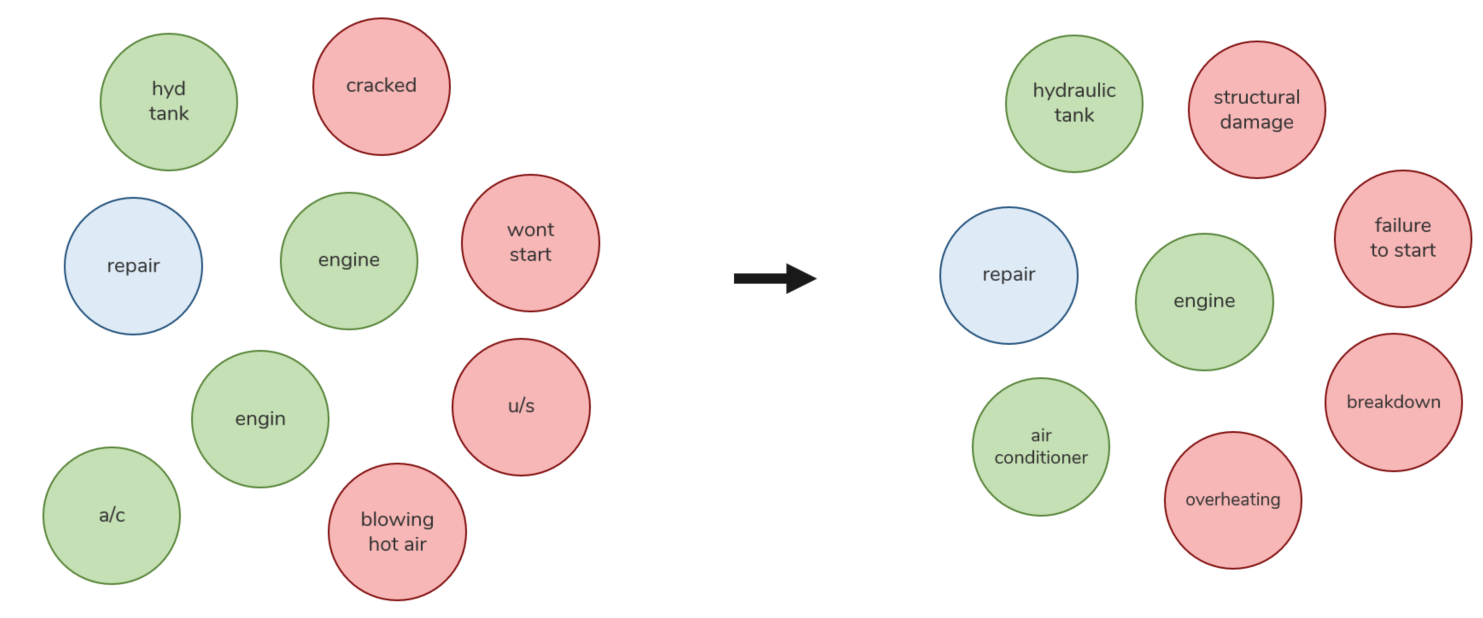
\includegraphics{images/normalising-entities.png}
\caption{alt text}
\end{figure}

    \begin{tcolorbox}[breakable, size=fbox, boxrule=1pt, pad at break*=1mm,colback=cellbackground, colframe=cellborder]
\prompt{In}{incolor}{76}{\boxspacing}
\begin{Verbatim}[commandchars=\\\{\}]
\PY{n}{lexicon\PYZus{}n\PYZus{}file} \PY{o}{=} \PY{l+s+s2}{\PYZdq{}}\PY{l+s+s2}{data/lexicon\PYZus{}normalisation.csv}\PY{l+s+s2}{\PYZdq{}}
\PY{n}{lexicon\PYZus{}normaliser} \PY{o}{=} \PY{n}{LexiconTagger}\PY{p}{(}\PY{n}{lexicon\PYZus{}n\PYZus{}file}\PY{p}{)}

\PY{n}{normalised\PYZus{}work\PYZus{}order\PYZus{}entities} \PY{o}{=} \PY{p}{[}\PY{p}{]}

\PY{c+c1}{\PYZsh{} For every row in work\PYZus{}order\PYZus{}entities, replace each ngram with its normalised counterpart}
\PY{c+c1}{\PYZsh{} as per the normalisation lexicon.}
\PY{c+c1}{\PYZsh{} For example, \PYZdq{}engin\PYZdq{} will become \PYZdq{}engine\PYZdq{}, \PYZdq{}leaking\PYZdq{} will become \PYZdq{}leak\PYZdq{}, etc.}
\PY{k}{for} \PY{n}{row} \PY{o+ow}{in} \PY{n}{work\PYZus{}order\PYZus{}entities}\PY{p}{:}
    \PY{n}{normalised\PYZus{}work\PYZus{}order\PYZus{}entities}\PY{o}{.}\PY{n}{append}\PY{p}{(}\PY{p}{[}\PY{p}{(}\PY{n}{lexicon\PYZus{}normaliser}\PY{o}{.}\PY{n}{normalise\PYZus{}ngram}\PY{p}{(}\PY{n}{ngram}\PY{p}{)}\PY{p}{,} \PY{n}{entity\PYZus{}class}\PY{p}{)} 
                                           \PY{k}{for} \PY{p}{(}\PY{n}{ngram}\PY{p}{,} \PY{n}{entity\PYZus{}class}\PY{p}{)} \PY{o+ow}{in} \PY{n}{row}\PY{p}{]}\PY{p}{)}
    
    
\PY{k}{for} \PY{n}{row} \PY{o+ow}{in} \PY{n}{normalised\PYZus{}work\PYZus{}order\PYZus{}entities}\PY{p}{:}
    \PY{n+nb}{print}\PY{p}{(}\PY{n}{row}\PY{p}{)}
\end{Verbatim}
\end{tcolorbox}

    \begin{Verbatim}[commandchars=\\\{\}]
[('repair', 'activity'), ('cracked', 'observation'), ('hydraulic tank', 'item')]
[('engine', 'item'), ('failure to start', 'observation')]
[('air conditioner', 'item'), ('overheating', 'observation')]
[('engine', 'item'), ('breakdown', 'observation')]
[('fix', 'activity'), ('engine', 'item')]
[('pump', 'item'), ('service', 'activity')]
[('pump', 'item'), ('leak', 'observation')]
[('fix', 'activity'), ('leak', 'observation'), ('pump', 'item')]
[('engine', 'item'), ('breakdown', 'observation')]
[('engine', 'item'), ('failure to start', 'observation')]
[('pump', 'item'), ('electrical issue', 'observation')]
[('pump', 'item'), ('leak', 'observation')]
[('air conditioner', 'item'), ('breakdown', 'observation')]
[('air conditioner', 'item'), ('breakdown', 'observation')]
    \end{Verbatim}

    \hypertarget{extract-relations-between-the-entities}{%
\subsection{Extract relations between the
entities}\label{extract-relations-between-the-entities}}

Now that we have our normalised set of (ngram, entity\_class) pairs for
each work order, we need to build the relationships between them.

In our graph we are going to link each ``item'' to every other entity
appearing in the work order.

\begin{figure}
\centering
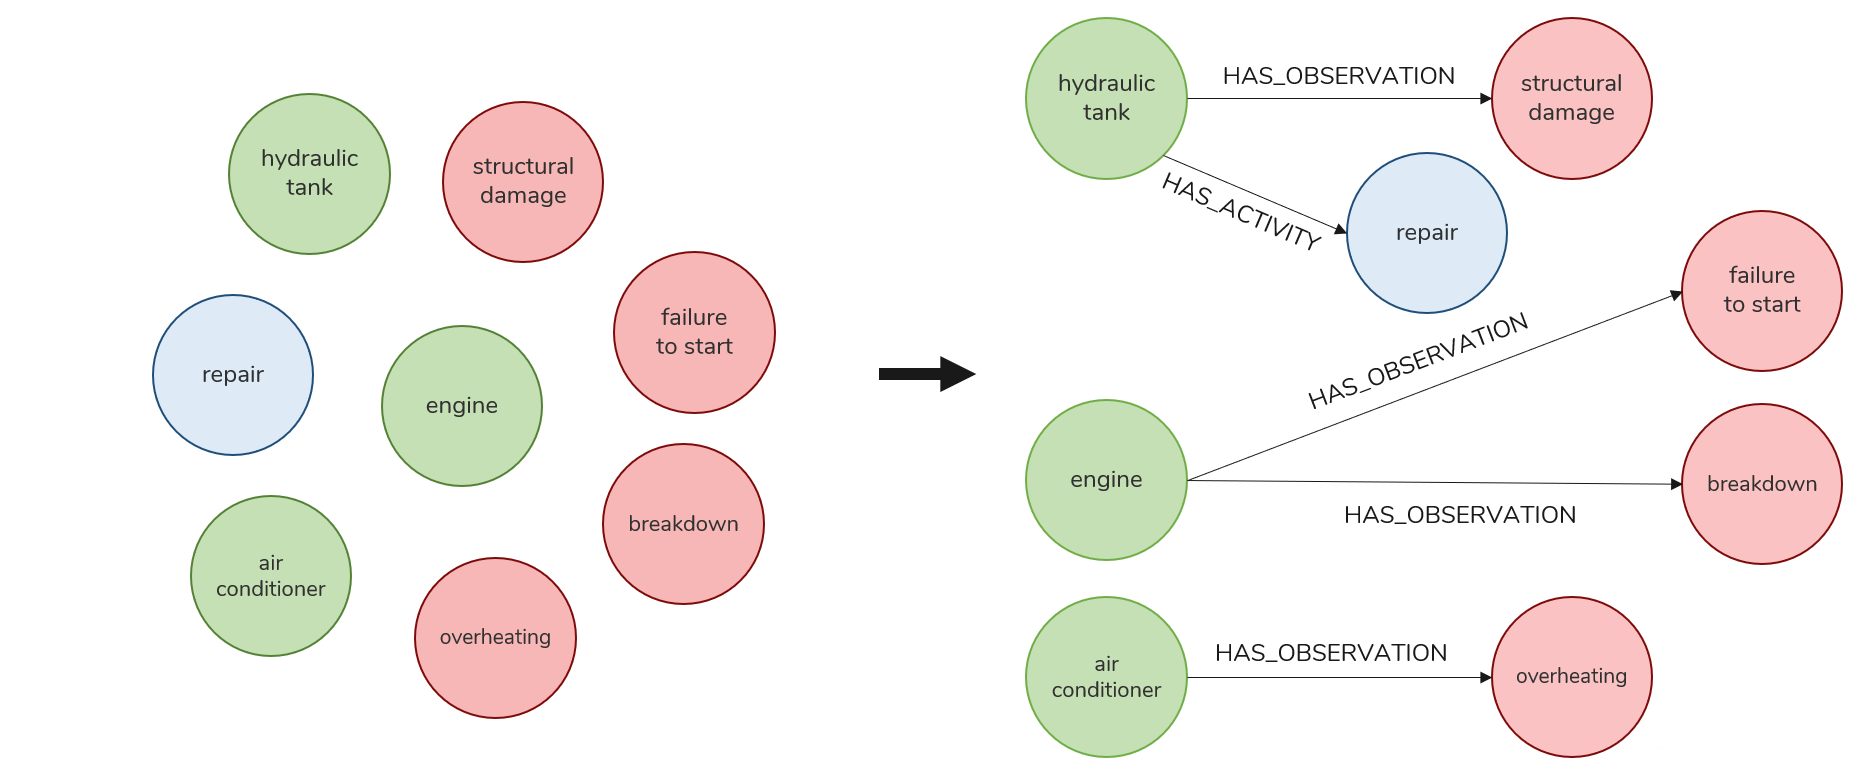
\includegraphics{images/building-relations.png}
\caption{alt text}
\end{figure}

    \begin{tcolorbox}[breakable, size=fbox, boxrule=1pt, pad at break*=1mm,colback=cellbackground, colframe=cellborder]
\prompt{In}{incolor}{77}{\boxspacing}
\begin{Verbatim}[commandchars=\\\{\}]
\PY{n}{triples} \PY{o}{=} \PY{p}{[}\PY{p}{]}

\PY{k}{for} \PY{n}{row} \PY{o+ow}{in} \PY{n}{normalised\PYZus{}work\PYZus{}order\PYZus{}entities}\PY{p}{:}
    \PY{k}{for} \PY{p}{(}\PY{n}{ngram}\PY{p}{,} \PY{n}{entity\PYZus{}class}\PY{p}{)} \PY{o+ow}{in} \PY{n}{row}\PY{p}{:}
        \PY{k}{if} \PY{n}{entity\PYZus{}class} \PY{o}{!=} \PY{l+s+s2}{\PYZdq{}}\PY{l+s+s2}{item}\PY{l+s+s2}{\PYZdq{}}\PY{p}{:} \PY{k}{continue}
            
        \PY{c+c1}{\PYZsh{} If this entity is an item, link it to all other entities in the work order       }
             
        \PY{k}{for} \PY{p}{(}\PY{n}{other\PYZus{}ngram}\PY{p}{,} \PY{n}{other\PYZus{}entity\PYZus{}class}\PY{p}{)} \PY{o+ow}{in} \PY{n}{row}\PY{p}{:}   
            \PY{k}{if} \PY{n}{ngram} \PY{o}{==} \PY{n}{other\PYZus{}ngram}\PY{p}{:} \PY{k}{continue} \PY{c+c1}{\PYZsh{} Don\PYZsq{}t link items to themselves                }

            \PY{n}{relation\PYZus{}type} \PY{o}{=} \PY{n}{other\PYZus{}entity\PYZus{}class}\PY{o}{.}\PY{n}{upper}\PY{p}{(}\PY{p}{)}                
            \PY{n}{triples}\PY{o}{.}\PY{n}{append}\PY{p}{(}\PY{p}{(}\PY{p}{(}\PY{n}{ngram}\PY{p}{,} \PY{n}{entity\PYZus{}class}\PY{p}{)}\PY{p}{,} \PY{l+s+s2}{\PYZdq{}}\PY{l+s+s2}{HAS\PYZus{}}\PY{l+s+si}{\PYZpc{}s}\PY{l+s+s2}{\PYZdq{}} \PY{o}{\PYZpc{}} \PY{n}{relation\PYZus{}type}\PY{p}{,} \PY{p}{(}\PY{n}{other\PYZus{}ngram}\PY{p}{,} \PY{n}{other\PYZus{}entity\PYZus{}class}\PY{p}{)}\PY{p}{)}\PY{p}{)}
        
\PY{k}{for} \PY{n}{triple} \PY{o+ow}{in} \PY{n}{triples}\PY{p}{:}
    \PY{n+nb}{print}\PY{p}{(}\PY{n}{triple}\PY{p}{)}
\end{Verbatim}
\end{tcolorbox}

    \begin{Verbatim}[commandchars=\\\{\}]
(('hydraulic tank', 'item'), 'HAS\_ACTIVITY', ('repair', 'activity'))
(('hydraulic tank', 'item'), 'HAS\_OBSERVATION', ('cracked', 'observation'))
(('engine', 'item'), 'HAS\_OBSERVATION', ('failure to start', 'observation'))
(('air conditioner', 'item'), 'HAS\_OBSERVATION', ('overheating', 'observation'))
(('engine', 'item'), 'HAS\_OBSERVATION', ('breakdown', 'observation'))
(('engine', 'item'), 'HAS\_ACTIVITY', ('fix', 'activity'))
(('pump', 'item'), 'HAS\_ACTIVITY', ('service', 'activity'))
(('pump', 'item'), 'HAS\_OBSERVATION', ('leak', 'observation'))
(('pump', 'item'), 'HAS\_ACTIVITY', ('fix', 'activity'))
(('pump', 'item'), 'HAS\_OBSERVATION', ('leak', 'observation'))
(('engine', 'item'), 'HAS\_OBSERVATION', ('breakdown', 'observation'))
(('engine', 'item'), 'HAS\_OBSERVATION', ('failure to start', 'observation'))
(('pump', 'item'), 'HAS\_OBSERVATION', ('electrical issue', 'observation'))
(('pump', 'item'), 'HAS\_OBSERVATION', ('leak', 'observation'))
(('air conditioner', 'item'), 'HAS\_OBSERVATION', ('breakdown', 'observation'))
(('air conditioner', 'item'), 'HAS\_OBSERVATION', ('breakdown', 'observation'))
    \end{Verbatim}

    \hypertarget{create-the-graph}{%
\section{Create the graph}\label{create-the-graph}}

Now that we have our nodes and relations we can go ahead and build the
Neo4J graph.

To do this we are going to use py2neo, a Python library for interacting
with Neo4J.

There are also a couple of other ways to do this - you can either use
Neo4J and run Cypher queries to insert each node and relation, or use
the APOC library to import a list of nodes from a CSV file. I find
Python to be the simplest way, however.

\begin{quote}
Before proceeding, make sure you have created a new graph in Neo4j and
that your new Neo4j graph is running.
\end{quote}

You can download and install Neo4j from here if you haven't already:
https://neo4j.com/download/. I will be demonstrating the graph during
the class so there's no need to have it installed unless you are also
interested in trying out some graph queries yourself.

\begin{quote}
If you need to build your graph again, make sure to run this cell before
running subsequent cells.
\end{quote}

    \begin{tcolorbox}[breakable, size=fbox, boxrule=1pt, pad at break*=1mm,colback=cellbackground, colframe=cellborder]
\prompt{In}{incolor}{78}{\boxspacing}
\begin{Verbatim}[commandchars=\\\{\}]
\PY{k+kn}{from} \PY{n+nn}{py2neo} \PY{k}{import} \PY{n}{Graph}
\PY{k+kn}{from} \PY{n+nn}{py2neo}\PY{n+nn}{.}\PY{n+nn}{data} \PY{k}{import} \PY{n}{Node}\PY{p}{,} \PY{n}{Relationship}

\PY{n}{GRAPH\PYZus{}PASSWORD} \PY{o}{=} \PY{l+s+s2}{\PYZdq{}}\PY{l+s+s2}{password}\PY{l+s+s2}{\PYZdq{}} \PY{c+c1}{\PYZsh{} Set this to the password of your Neo4J graph}

\PY{n}{graph} \PY{o}{=} \PY{n}{Graph}\PY{p}{(}\PY{n}{password} \PY{o}{=} \PY{n}{GRAPH\PYZus{}PASSWORD}\PY{p}{)}

\PY{c+c1}{\PYZsh{} We will start by deleting all nodes and edges in the current graph.}
\PY{c+c1}{\PYZsh{} If we don\PYZsq{}t do this, we will end up with duplicate nodes and edges when running this script again.}
\PY{n}{graph}\PY{o}{.}\PY{n}{delete\PYZus{}all}\PY{p}{(}\PY{p}{)} 

\PY{n}{tx} \PY{o}{=} \PY{n}{graph}\PY{o}{.}\PY{n}{begin}\PY{p}{(}\PY{p}{)}

\PY{c+c1}{\PYZsh{} We will keep a dictionary of nodes that we have created so far.}
\PY{c+c1}{\PYZsh{} This serves two purposes:}
\PY{c+c1}{\PYZsh{}  \PYZhy{} prevents duplicate nodes}
\PY{c+c1}{\PYZsh{}  \PYZhy{} provides us with a way to create edges between the nodes}
\PY{n}{created\PYZus{}entity\PYZus{}nodes} \PY{o}{=} \PY{p}{\PYZob{}}\PY{p}{\PYZcb{}}

\PY{c+c1}{\PYZsh{} Creates a node for the specified ngram and entity\PYZus{}class.}
\PY{c+c1}{\PYZsh{} If the node has already been created (i.e. it exists in created\PYZus{}nodes), return the node.}
\PY{c+c1}{\PYZsh{} Otherwise, create a new one.}
\PY{k}{def} \PY{n+nf}{create\PYZus{}entity\PYZus{}node}\PY{p}{(}\PY{n}{ngram}\PY{p}{,} \PY{n}{entity\PYZus{}class}\PY{p}{)}\PY{p}{:}
    \PY{k}{if} \PY{n}{ngram} \PY{o+ow}{in} \PY{n}{created\PYZus{}entity\PYZus{}nodes}\PY{p}{:}
        \PY{n}{node} \PY{o}{=} \PY{n}{created\PYZus{}entity\PYZus{}nodes}\PY{p}{[}\PY{n}{ngram}\PY{p}{]}
    \PY{k}{else}\PY{p}{:}
        \PY{n}{node} \PY{o}{=} \PY{n}{Node}\PY{p}{(}\PY{l+s+s2}{\PYZdq{}}\PY{l+s+s2}{Entity}\PY{l+s+s2}{\PYZdq{}}\PY{p}{,} \PY{n}{entity\PYZus{}class}\PY{p}{,} \PY{n}{name}\PY{o}{=}\PY{n}{ngram}\PY{p}{)}
        \PY{n}{created\PYZus{}entity\PYZus{}nodes}\PY{p}{[}\PY{n}{ngram}\PY{p}{]} \PY{o}{=} \PY{n}{node}
        \PY{n}{tx}\PY{o}{.}\PY{n}{create}\PY{p}{(}\PY{n}{node}\PY{p}{)}
    \PY{k}{return} \PY{n}{node}


\PY{c+c1}{\PYZsh{} Create a node for each triple in the list of triples.}
\PY{c+c1}{\PYZsh{} Set the class of each node to the entity\PYZus{}class (e.g. \PYZdq{}activity\PYZdq{}, \PYZdq{}item\PYZdq{} or \PYZdq{}observation\PYZdq{}).}
\PY{c+c1}{\PYZsh{} Create a relationship between the nodes in the triple.}
\PY{k}{for} \PY{p}{(}\PY{p}{(}\PY{n}{ngram\PYZus{}1}\PY{p}{,} \PY{n}{entity\PYZus{}class\PYZus{}1}\PY{p}{)}\PY{p}{,} \PY{n}{relation}\PY{p}{,} \PY{p}{(}\PY{n}{ngram\PYZus{}2}\PY{p}{,} \PY{n}{entity\PYZus{}class\PYZus{}2}\PY{p}{)}\PY{p}{)} \PY{o+ow}{in} \PY{n}{triples}\PY{p}{:}
    
    \PY{n}{node\PYZus{}1} \PY{o}{=} \PY{n}{create\PYZus{}entity\PYZus{}node}\PY{p}{(}\PY{n}{ngram\PYZus{}1}\PY{p}{,} \PY{n}{entity\PYZus{}class\PYZus{}1}\PY{p}{)}
    \PY{n}{node\PYZus{}2} \PY{o}{=} \PY{n}{create\PYZus{}entity\PYZus{}node}\PY{p}{(}\PY{n}{ngram\PYZus{}2}\PY{p}{,} \PY{n}{entity\PYZus{}class\PYZus{}2}\PY{p}{)}   
    
    
    \PY{c+c1}{\PYZsh{} Create a relationship between two nodes.}
    \PY{c+c1}{\PYZsh{} This does not check for duplicate relationships unlike create\PYZus{}node,}
    \PY{c+c1}{\PYZsh{} so this code will need to be adjusted on larger datasets.}
    \PY{n}{relationship} \PY{o}{=} \PY{n}{Relationship}\PY{p}{(} \PY{n}{node\PYZus{}1}\PY{p}{,} \PY{n}{relation}\PY{p}{,} \PY{n}{node\PYZus{}2} \PY{p}{)}
    \PY{n}{tx}\PY{o}{.}\PY{n}{create}\PY{p}{(}\PY{n}{relationship}\PY{p}{)}
    
    
\PY{n}{tx}\PY{o}{.}\PY{n}{commit}\PY{p}{(}\PY{p}{)}
        
\end{Verbatim}
\end{tcolorbox}

    \hypertarget{create-nodes-for-the-work-orders}{%
\subsection{Create nodes for the work
orders}\label{create-nodes-for-the-work-orders}}

In order to query our graph, we need to create nodes for each work order
in our dataset as well. We then need to link each Document node to every
Entity node appearing in that document.

    \begin{tcolorbox}[breakable, size=fbox, boxrule=1pt, pad at break*=1mm,colback=cellbackground, colframe=cellborder]
\prompt{In}{incolor}{79}{\boxspacing}
\begin{Verbatim}[commandchars=\\\{\}]
\PY{k+kn}{from} \PY{n+nn}{dateutil}\PY{n+nn}{.}\PY{n+nn}{parser} \PY{k}{import} \PY{n}{parse} \PY{k}{as} \PY{n}{parse\PYZus{}date}

\PY{c+c1}{\PYZsh{} Our work\PYZus{}order\PYZus{}data and normalised\PYZus{}work\PYZus{}order entities allow us to do this quite easily,}

\PY{n}{tx} \PY{o}{=} \PY{n}{graph}\PY{o}{.}\PY{n}{begin}\PY{p}{(}\PY{p}{)}

\PY{c+c1}{\PYZsh{} We will once again keep a mapping of created work order nodes, this time indexed by the row index.}
\PY{n}{created\PYZus{}work\PYZus{}order\PYZus{}nodes} \PY{o}{=} \PY{p}{\PYZob{}}\PY{p}{\PYZcb{}}

\PY{c+c1}{\PYZsh{} Dates are a little awkward in Neo4j \PYZhy{} we have to convert it to an integer representation in Python.}
\PY{c+c1}{\PYZsh{} The APOC library has functions to handle this better.}
\PY{k}{def} \PY{n+nf}{date\PYZus{}to\PYZus{}int}\PY{p}{(}\PY{n}{date}\PY{p}{)}\PY{p}{:}
    \PY{n}{parsed\PYZus{}date} \PY{o}{=} \PY{n}{parse\PYZus{}date}\PY{p}{(}\PY{n+nb}{str}\PY{p}{(}\PY{n}{date}\PY{p}{)}\PY{p}{)}
    \PY{n}{date} \PY{o}{=} \PY{n+nb}{int}\PY{p}{(}\PY{l+s+s2}{\PYZdq{}}\PY{l+s+si}{\PYZpc{}s}\PY{l+s+si}{\PYZpc{}s}\PY{l+s+si}{\PYZpc{}s}\PY{l+s+s2}{\PYZdq{}} \PY{o}{\PYZpc{}} \PY{p}{(}\PY{n}{parsed\PYZus{}date}\PY{o}{.}\PY{n}{year}\PY{p}{,} \PY{n+nb}{str}\PY{p}{(}\PY{n}{parsed\PYZus{}date}\PY{o}{.}\PY{n}{month}\PY{p}{)}\PY{o}{.}\PY{n}{zfill}\PY{p}{(}\PY{l+m+mi}{2}\PY{p}{)}\PY{p}{,} \PY{n+nb}{str}\PY{p}{(}\PY{n}{parsed\PYZus{}date}\PY{o}{.}\PY{n}{day}\PY{p}{)}\PY{o}{.}\PY{n}{zfill}\PY{p}{(}\PY{l+m+mi}{2}\PY{p}{)}\PY{p}{)}\PY{p}{)}
    \PY{k}{return} \PY{n}{date}

\PY{c+c1}{\PYZsh{} The process of creating a work order node is a bit different to creating an entity,}
\PY{c+c1}{\PYZsh{} as we also want to incorporate some of the structured fields onto the node.}
\PY{k}{def} \PY{n+nf}{create\PYZus{}structured\PYZus{}node}\PY{p}{(}\PY{n}{index}\PY{p}{,} \PY{n}{row}\PY{p}{,} \PY{n}{node\PYZus{}type}\PY{p}{,} \PY{n}{created\PYZus{}nodes}\PY{p}{)}\PY{p}{:}
    \PY{k}{if} \PY{n}{index} \PY{o+ow}{in} \PY{n}{created\PYZus{}nodes}\PY{p}{:}
        \PY{k}{return} \PY{n}{created\PYZus{}nodes}\PY{p}{[}\PY{n}{index}\PY{p}{]}

    \PY{k}{if} \PY{l+s+s1}{\PYZsq{}}\PY{l+s+s1}{StartDate}\PY{l+s+s1}{\PYZsq{}} \PY{o+ow}{in} \PY{n}{row}\PY{p}{:}
        \PY{n}{row}\PY{p}{[}\PY{l+s+s1}{\PYZsq{}}\PY{l+s+s1}{StartDate}\PY{l+s+s1}{\PYZsq{}}\PY{p}{]} \PY{o}{=} \PY{n}{date\PYZus{}to\PYZus{}int}\PY{p}{(}\PY{n}{row}\PY{p}{[}\PY{l+s+s1}{\PYZsq{}}\PY{l+s+s1}{StartDate}\PY{l+s+s1}{\PYZsq{}}\PY{p}{]}\PY{p}{)}
    \PY{k}{if} \PY{l+s+s1}{\PYZsq{}}\PY{l+s+s1}{EndDate}\PY{l+s+s1}{\PYZsq{}} \PY{o+ow}{in} \PY{n}{row}\PY{p}{:}
        \PY{n}{row}\PY{p}{[}\PY{l+s+s1}{\PYZsq{}}\PY{l+s+s1}{EndDate}\PY{l+s+s1}{\PYZsq{}}\PY{p}{]} \PY{o}{=} \PY{n}{date\PYZus{}to\PYZus{}int}\PY{p}{(}\PY{n}{row}\PY{p}{[}\PY{l+s+s1}{\PYZsq{}}\PY{l+s+s1}{EndDate}\PY{l+s+s1}{\PYZsq{}}\PY{p}{]}\PY{p}{)}  

    \PY{n}{node} \PY{o}{=} \PY{n}{Node}\PY{p}{(}\PY{n}{node\PYZus{}type}\PY{p}{,} \PY{o}{*}\PY{o}{*}\PY{n}{row}\PY{p}{)}
    \PY{n}{created\PYZus{}nodes}\PY{p}{[}\PY{n}{index}\PY{p}{]} \PY{o}{=} \PY{n}{node}
    \PY{n}{tx}\PY{o}{.}\PY{n}{create}\PY{p}{(}\PY{n}{node}\PY{p}{)}
    \PY{k}{return} \PY{n}{node}

\PY{k}{for} \PY{n}{i}\PY{p}{,} \PY{n}{row} \PY{o+ow}{in} \PY{n+nb}{enumerate}\PY{p}{(}\PY{n}{work\PYZus{}order\PYZus{}data}\PY{p}{)}\PY{p}{:}
    \PY{n}{node} \PY{o}{=} \PY{n}{create\PYZus{}structured\PYZus{}node}\PY{p}{(}\PY{n}{i}\PY{p}{,} \PY{n}{row}\PY{p}{,} \PY{l+s+s2}{\PYZdq{}}\PY{l+s+s2}{WorkOrder}\PY{l+s+s2}{\PYZdq{}}\PY{p}{,} \PY{n}{created\PYZus{}work\PYZus{}order\PYZus{}nodes}\PY{p}{)}
    
\PY{n}{tx}\PY{o}{.}\PY{n}{commit}\PY{p}{(}\PY{p}{)}
\end{Verbatim}
\end{tcolorbox}

    \hypertarget{link-the-entities-to-their-corresponding-work-order-nodes}{%
\subsection{3.2 Link the entities to their corresponding work order
nodes}\label{link-the-entities-to-their-corresponding-work-order-nodes}}

In order to properly query our graph, we need to link every entity node
to the work order node in which it appears.

This allows us to run queries such as ``pumps with electrical issues in
the last 3 months''.

    \begin{tcolorbox}[breakable, size=fbox, boxrule=1pt, pad at break*=1mm,colback=cellbackground, colframe=cellborder]
\prompt{In}{incolor}{80}{\boxspacing}
\begin{Verbatim}[commandchars=\\\{\}]
\PY{n}{tx} \PY{o}{=} \PY{n}{graph}\PY{o}{.}\PY{n}{begin}\PY{p}{(}\PY{p}{)}

\PY{c+c1}{\PYZsh{} We can use the normalised\PYZus{}work\PYZus{}order\PYZus{}entries list to do this.}
\PY{k}{for} \PY{n}{i}\PY{p}{,} \PY{n}{row} \PY{o+ow}{in} \PY{n+nb}{enumerate}\PY{p}{(}\PY{n}{normalised\PYZus{}work\PYZus{}order\PYZus{}entities}\PY{p}{)}\PY{p}{:}
    \PY{k}{for} \PY{p}{(}\PY{n}{ngram}\PY{p}{,} \PY{n}{entity\PYZus{}class}\PY{p}{)} \PY{o+ow}{in} \PY{n}{row}\PY{p}{:}        
        
        \PY{n}{node\PYZus{}1} \PY{o}{=} \PY{n}{created\PYZus{}entity\PYZus{}nodes}\PY{p}{[}\PY{n}{ngram}\PY{p}{]}
        \PY{n}{node\PYZus{}2} \PY{o}{=} \PY{n}{created\PYZus{}work\PYZus{}order\PYZus{}nodes}\PY{p}{[}\PY{n}{i}\PY{p}{]}
        
        \PY{n}{relationship} \PY{o}{=} \PY{n}{Relationship}\PY{p}{(} \PY{n}{node\PYZus{}1}\PY{p}{,} \PY{l+s+s2}{\PYZdq{}}\PY{l+s+s2}{APPEARS\PYZus{}IN}\PY{l+s+s2}{\PYZdq{}}\PY{p}{,} \PY{n}{node\PYZus{}2} \PY{p}{)}
        \PY{n}{tx}\PY{o}{.}\PY{n}{create}\PY{p}{(}\PY{n}{relationship}\PY{p}{)}
       
\PY{n}{tx}\PY{o}{.}\PY{n}{commit}\PY{p}{(}\PY{p}{)}
\end{Verbatim}
\end{tcolorbox}

    \hypertarget{extending-the-graph-to-incorporate-downtime-events}{%
\section{4. Extending the graph to incorporate Downtime
events}\label{extending-the-graph-to-incorporate-downtime-events}}

The next step is to incorporate the downtime events.

For this exercise we are going to link the Downtime events to the first
Item node appearing in the work orders with the same FLOC as the
downtime event.

\begin{figure}
\centering
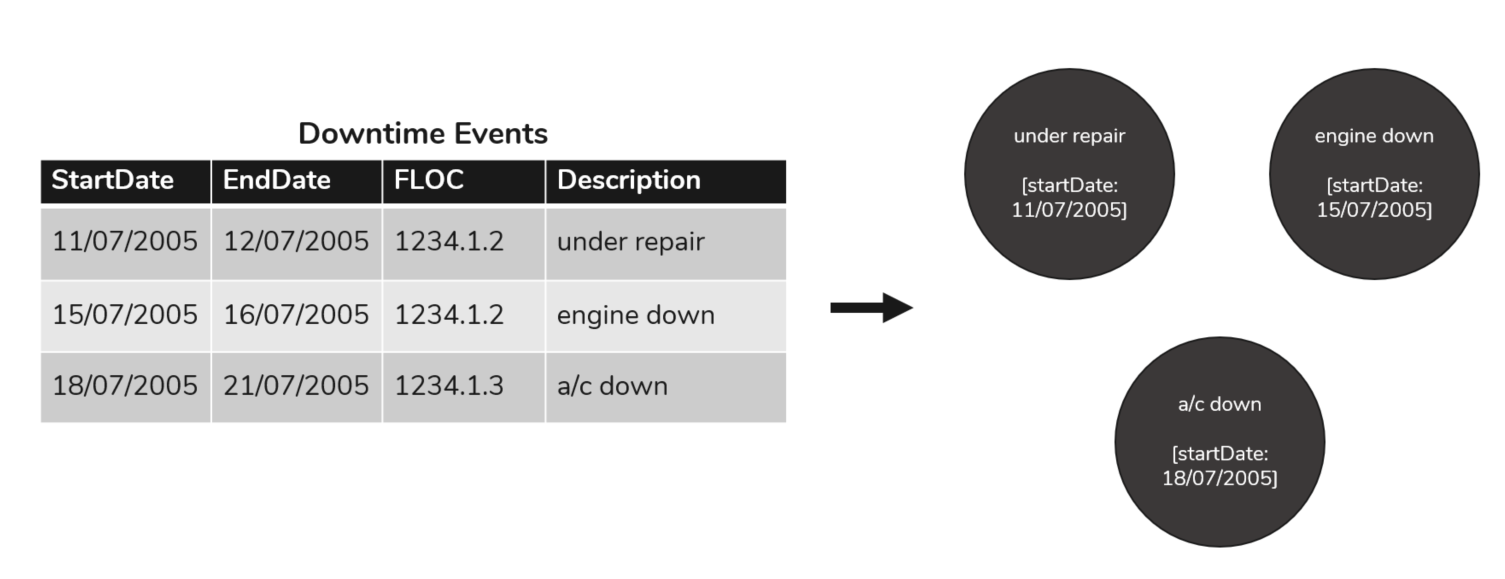
\includegraphics{images/adding-downtime-events.png}
\caption{alt text}
\end{figure}

    \begin{tcolorbox}[breakable, size=fbox, boxrule=1pt, pad at break*=1mm,colback=cellbackground, colframe=cellborder]
\prompt{In}{incolor}{81}{\boxspacing}
\begin{Verbatim}[commandchars=\\\{\}]
\PY{n}{tx} \PY{o}{=} \PY{n}{graph}\PY{o}{.}\PY{n}{begin}\PY{p}{(}\PY{p}{)}

\PY{n}{created\PYZus{}downtime\PYZus{}nodes} \PY{o}{=} \PY{p}{\PYZob{}}\PY{p}{\PYZcb{}}

\PY{c+c1}{\PYZsh{} Create a DowntimeEvent node for each row}
\PY{k}{for} \PY{n}{i}\PY{p}{,} \PY{n}{downtime\PYZus{}row} \PY{o+ow}{in} \PY{n+nb}{enumerate}\PY{p}{(}\PY{n}{downtime\PYZus{}data}\PY{p}{)}\PY{p}{:}
    \PY{n}{node} \PY{o}{=} \PY{n}{create\PYZus{}structured\PYZus{}node}\PY{p}{(}\PY{n}{i}\PY{p}{,} \PY{n}{downtime\PYZus{}row}\PY{p}{,} \PY{l+s+s2}{\PYZdq{}}\PY{l+s+s2}{DowntimeEvent}\PY{l+s+s2}{\PYZdq{}}\PY{p}{,} \PY{n}{created\PYZus{}downtime\PYZus{}nodes}\PY{p}{)}
    
    \PY{c+c1}{\PYZsh{} Get all work order nodes with the same FLOC and link the DowntimeEvent to the Items appearing}
    \PY{c+c1}{\PYZsh{} in those work orders}
    \PY{k}{for} \PY{n}{j}\PY{p}{,} \PY{n}{work\PYZus{}order\PYZus{}row} \PY{o+ow}{in} \PY{n+nb}{enumerate}\PY{p}{(}\PY{n}{work\PYZus{}order\PYZus{}data}\PY{p}{)}\PY{p}{:}
        \PY{k}{if} \PY{n}{work\PYZus{}order\PYZus{}row}\PY{p}{[}\PY{l+s+s2}{\PYZdq{}}\PY{l+s+s2}{FLOC}\PY{l+s+s2}{\PYZdq{}}\PY{p}{]} \PY{o}{==} \PY{n}{downtime\PYZus{}row}\PY{p}{[}\PY{l+s+s2}{\PYZdq{}}\PY{l+s+s2}{FLOC}\PY{l+s+s2}{\PYZdq{}}\PY{p}{]}\PY{p}{:}
            
            \PY{n}{work\PYZus{}order\PYZus{}entities} \PY{o}{=} \PY{n}{normalised\PYZus{}work\PYZus{}order\PYZus{}entities}\PY{p}{[}\PY{n}{j}\PY{p}{]}
            
            \PY{k}{for} \PY{p}{(}\PY{n}{ngram}\PY{p}{,} \PY{n}{entity\PYZus{}class}\PY{p}{)} \PY{o+ow}{in} \PY{n}{work\PYZus{}order\PYZus{}entities}\PY{p}{:}
                \PY{k}{if} \PY{n}{entity\PYZus{}class} \PY{o}{!=} \PY{l+s+s2}{\PYZdq{}}\PY{l+s+s2}{item}\PY{l+s+s2}{\PYZdq{}}\PY{p}{:} \PY{k}{continue}    \PY{c+c1}{\PYZsh{} We don\PYZsq{}t need to link non\PYZhy{}items to downtime events               }
                    
                \PY{n}{item\PYZus{}node} \PY{o}{=} \PY{n}{created\PYZus{}entity\PYZus{}nodes}\PY{p}{[}\PY{n}{ngram}\PY{p}{]}
                \PY{n}{relationship} \PY{o}{=} \PY{n}{Relationship}\PY{p}{(} \PY{n}{item\PYZus{}node}\PY{p}{,} \PY{l+s+s2}{\PYZdq{}}\PY{l+s+s2}{HAS\PYZus{}EVENT}\PY{l+s+s2}{\PYZdq{}}\PY{p}{,} \PY{n}{node} \PY{p}{)}
                \PY{n}{tx}\PY{o}{.}\PY{n}{create}\PY{p}{(}\PY{n}{relationship}\PY{p}{)}
                \PY{k}{break}

    
\PY{n}{tx}\PY{o}{.}\PY{n}{commit}\PY{p}{(}\PY{p}{)}
\end{Verbatim}
\end{tcolorbox}

    \hypertarget{querying-the-graph}{%
\section{5. Querying the graph}\label{querying-the-graph}}

Now that the graph has been created, we can query it in Neo4j. This
section lists some example queries that we can run on our graph. If you
would like to try these yourself you can paste them directly into the
Neo4j console.

First, let's try a simple query. Here is a query that searches for
\textbf{all failure modes observed on engines}:

\begin{verbatim}
MATCH (e:Entity {name: "engine"})-[r:HAS_OBSERVATION]->(o:observation)
RETURN e, r, o
\end{verbatim}

We can also use our graph as a way to quickly search and access work
orders for the entities appearing in those work orders. For example,
searching for \textbf{all work orders containing a leak}:

\begin{verbatim}
MATCH (d:WorkOrder)<-[a:APPEARS_IN]-(o:observation {name: "leak"})
RETURN d, a, o
\end{verbatim}

We could extend this to also show the items on which the leaks were
present:

\begin{verbatim}
MATCH (d:WorkOrder)<-[a:APPEARS_IN]-(o:observation {name: "leak"})
<-[r:HAS_OBSERVATION]-(e:Entity)
RETURN d, a, o, r, e
\end{verbatim}

Our queries can also incorporate structured data, such as the start
dates of the work orders. Here is an example query for \textbf{all
assets that had leaks from 25 to 28 July}:

\begin{verbatim}
MATCH (d:WorkOrder)<-[a:APPEARS_IN]-(e:Entity)-[r:HAS_OBSERVATION]->
(o:observation {name: "leak"})-[:APPEARS_IN]->(d)
WHERE d.StartDate >= 20050725
AND d.StartDate <= 20050728
RETURN e, r, o
\end{verbatim}

On a larger graph this would also work well with other forms of
structured data such as costs. We could query based on specific asset
costs, for example.

Now that our work orders and downtime events are in one graph, we can
also make queries about downtime events. Here is an example query for
the \textbf{downtime events associated with assets appearing in work
orders from 25 to 28 July (where the downtime events occurred in July)}:

\begin{verbatim}
MATCH (d:WorkOrder)<-[a:APPEARS_IN]-(e:Entity)-[r:HAS_EVENT]->
(x:DowntimeEvent)
WHERE d.StartDate > 20050725
AND d.StartDate < 20050728
AND 20050700 <= x.StartDate <= 20050731
RETURN e, r, x
\end{verbatim}

We can of course extend this to specific assets, such as pumps:

\begin{verbatim}
MATCH (d:WorkOrder)<-[a:APPEARS_IN]-(e:Entity {name: "pump"})
-[r:HAS_EVENT]->(x:DowntimeEvent)
WHERE d.StartDate > 20050725
AND d.StartDate < 20050728
AND 20050700 <= x.StartDate <= 20050731
RETURN e, r, x
\end{verbatim}

In larger graphs the downtime events could even be further queried based
on duration, cost, lost feed, or date ranges.

    \hypertarget{future-improvements}{%
\section{6. Future improvements}\label{future-improvements}}

\hypertarget{incorporating-flocs}{%
\subsection{Incorporating FLOCs}\label{incorporating-flocs}}

Our downtime events are currently linked to Item nodes, but it would
make more sense to link them to nodes representing the functional
locations.

If you are interested in continuing work on this small graph, the next
best step would be to create nodes for the functional location data
(\texttt{floc\_data}) and to link the downtime events to those nodes as
opposed to the Item nodes.

\begin{figure}
\centering
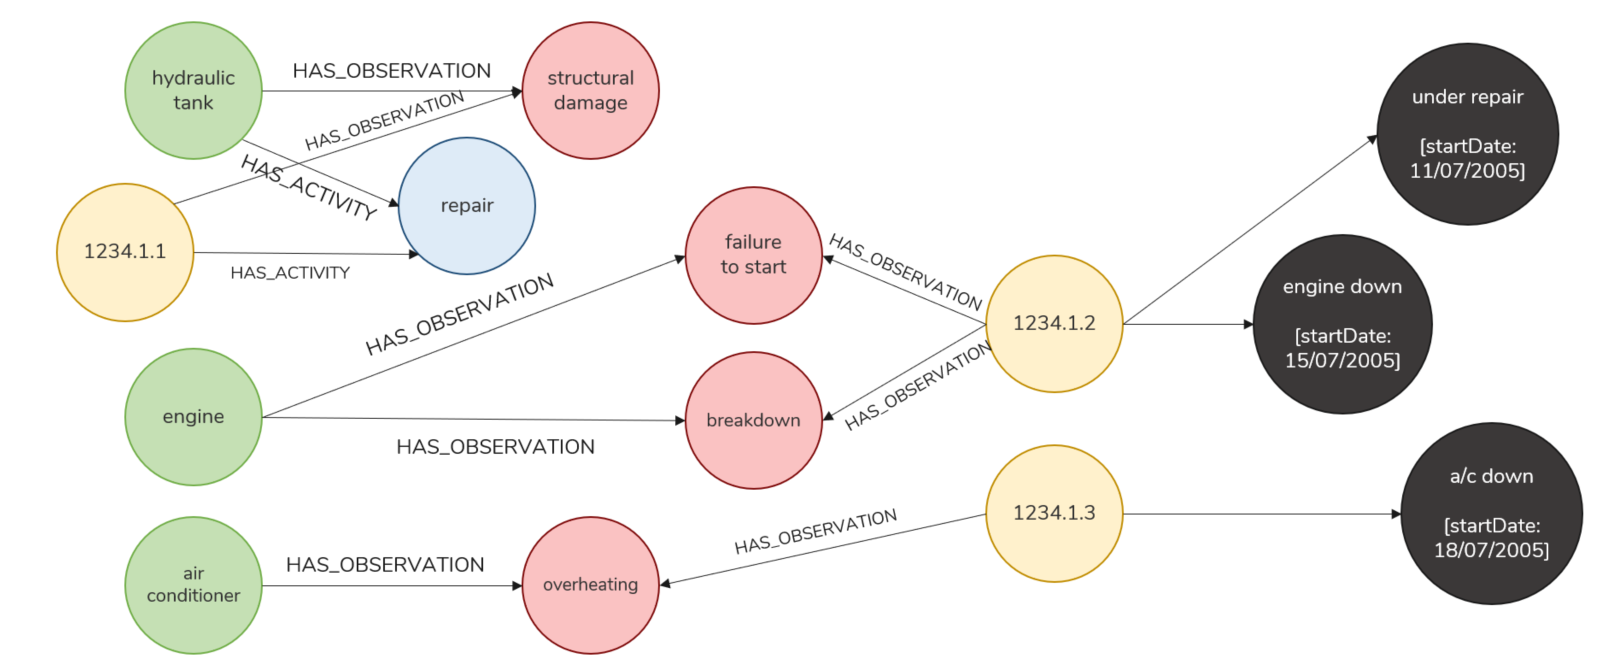
\includegraphics{images/adding-flocs.png}
\caption{alt text}
\end{figure}

\hypertarget{frequencies-on-edge-properties}{%
\subsection{Frequencies on edge
properties}\label{frequencies-on-edge-properties}}

We could also improve the graph by incorporating frequencies onto the
edge properties. For example, if a ``leak'' occurred on a pump in two
different work orders, our link between ``pump'' and ``leak'' could have
a property called \texttt{frequency} with a value of \texttt{2}. This
would allow us to query, for example, assets that had a particularly
high number of leaks.

\hypertarget{constructing-a-graph-from-your-own-work-order-data}{%
\subsection{Constructing a graph from your own work order
data}\label{constructing-a-graph-from-your-own-work-order-data}}

If you have a work order dataset of your own, feel free to download this
code and try it out on your dataset. I would be happy to chat if you would
like to further discuss the code or if you run into any issues.

If you need to extract entities not listed in the lexicon, you will need
to update the lexicon file to include your new entities. Alternatively,
the LexiconTagger can be substituted for a named entity recognition
model.

    \begin{tcolorbox}[breakable, size=fbox, boxrule=1pt, pad at break*=1mm,colback=cellbackground, colframe=cellborder]
\prompt{In}{incolor}{82}{\boxspacing}
\begin{Verbatim}[commandchars=\\\{\}]
\PY{n}{floc\PYZus{}file} \PY{o}{=} \PY{l+s+s2}{\PYZdq{}}\PY{l+s+s2}{data/sample\PYZus{}flocs.csv}\PY{l+s+s2}{\PYZdq{}}
\PY{n}{floc\PYZus{}data} \PY{o}{=} \PY{n}{load\PYZus{}csv}\PY{p}{(}\PY{n}{floc\PYZus{}file}\PY{p}{)}

\PY{c+c1}{\PYZsh{} Your code here}
\end{Verbatim}
\end{tcolorbox}


    % Add a bibliography block to the postdoc
    
    
    
\end{document}
